\documentclass{llncs}
\usepackage[utf8]{inputenc}
\usepackage{todonotes}
\usepackage{amsmath}
\usepackage[hidelinks]{hyperref}
\usepackage{cleveref}
\crefname{figure}{Fig.}{Fig.}
\usepackage{xstring}
\usepackage{booktabs}
\usepackage{tikz}
\usetikzlibrary{arrows,snakes,patterns,matrix,shapes,fit,calc,shadows,plotmarks,decorations.pathmorphing,decorations.markings,backgrounds}
\usetikzlibrary{external}
\tikzexternalize
\tikzsetexternalprefix{fig/}

\usepackage{pgfplots}
\pgfplotsset{compat=1.4, width=0.9\columnwidth, height=0.6\columnwidth}

\newcommand{\inputtikz}[1]
{
  \StrSubstitute{#1}{/}{.}[\fn]
  \scancs{\filename}{\fn}
  \tikzsetfigurename{\filename}
  \input{#1.tikz}
}

\renewcommand{\textfraction}{0.15}
\renewcommand{\topfraction}{0.85}
\renewcommand{\bottomfraction}{0.65}
\renewcommand{\floatpagefraction}{0.60}

\graphicspath{{fig/}}
%%%%%%%%%%%%%%%%%%%%%%%%%%%%%%%%%%%%%%%%%%%%%%%%%%%%%%%%%%%%%%%%%%%%%%%%%%%%%%%%
\begin{document}

\title{SimSpark: An Open Source Robot Simulator Developed by RoboCup Community}

\author{Yuan Xu\inst{1} \and Hedayat Vatankhah\inst{2}}

\institute{
\begin{minipage}[t]{0.4\textwidth}
\centering
DAI-Labor \\
Technische Universität Berlin \\
Ernst-Reuter-Platz 7, Berlin \\
D-10587 Germany\\
\email{yuan.xu@dai-labor.de}
\end{minipage}
\begin{minipage}[t]{0.4\textwidth}
\and
\centering
Department of Computer Engineering and IT \\
Amirkabir University of Technology \\
Tehran, Iran\\
\email{hedayatv@gmail.com}
\end{minipage}
}

\maketitle

\begin{abstract}
  SimSpark is an open source robot simulator developed by RoboCup Community.
  This paper briefly describes the development of SimSpark since 2008.
  Furthermore, some new features are proposed and implemented for the next RoboCup, including realistic motor, heterogeneous robots, and agent proxies.
  As a powerful tool to state different multi-robot researches, SimSpark has been successfully used in RoboCup simulation league, standard platform league and humanoid league.
\end{abstract}

\section{Introduction}
The development on robots may be severely limited by the constrained resources.
This is especially true in the research of multi-robot systems in areas such as RoboCup.
Using simulation for algorithm development and testing makes thing easier.

% \paragraph{History}
\textit{SimSpark}, a multi-robot simulator based on the generic components of the Spark\cite{OR05} physical multi-agent simulation system, has been used in the RoboCup Soccer Simulation League since 2004.
The project was registered as open source project in SourceForge in 2004, it has an established code base with development increasing year-over-year.
As the result, RoboCup soccer simulations have changed significantly over the years, going from rather abstract agent representations to more and more realistic humanoid robot games\cite{Boedecker2008,usermanual}.
Thanks to the flexibility of the Spark system, these transitions were achieved with little changes to the simulator's core architecture.

In this paper we describe the recent development of \textit{SimSpark} project, which make the \textit{SimSpark} possible to simulate 11 vs. 11 humanoid robot soccer games in real time\todo{is it real time in RoboCup 2012?}.
In section \ref{s:overview}, we will give an overview of \textit{SimSpark} project since 2008. After that, we will describe the development of the \textit{Spark} simulation platform in section \ref{s:spark}.
In section \ref{s:rcssserver3d}, we will briefly describe the implementation of RoboCup 3D Soccer Simulator -- \textit{RCSSServer3D}.
We will introduce some new features for RoboCup 2013 in section \ref{s:ongoing}.
Furthermore, we will discuss the application of \textit{SimSpark} not only in simulation league but also other leagues with real robots in section \ref{s:application}.
Finally, we will outline future development plans in section \ref{s:conclusion}.

\section{Project Overview}
\label{s:overview}

Until 2008, soccer simulation and SimSpark simulator were developed and released as a single project called rcssserver3d, but it was already decided that they should be separated 
to make the separation more visible for both users and developers.
In late 2008, the separation happened with the migration of sources from CVS repository
at \url{http://sserver.sourceforge.net} to SimSpark's project Subversion repository at 
\url{http://simspark.sourceforge.net}. As part of this process, the project was broken
to two main projects (Spark simulation platform and RCSSServer3D soccer simulation server) 
and two auxiliary projects (RSGEdit and simspark-utilities). Also, simspark binary was 
renamed to rcssserver3d to make it clear that it runs soccer simulation rather than a 
generic simulation environment.

SimSpark was never a single-platform project, but it practically didn't support 
Windows. In recent years, Windows support was added after migration from Autotools
to CMake, and windows installers are now released. 

\section{Spark}
\label{s:spark}
As a generic simulation environment, Spark provides a rich set of features to create, debug and modify multi-robot simulation.
It has three main components, including the simulation engine, the object and memory management system, and the physics engine. Details about architecture and concepts of Spark have been described in \cite{Boedecker2008,OR05}.
In this section, we describe the necessary changes for simulating 11 vs. 11 humanoid robot soccer game.
However changes to the simulator core were never customized for the soccer simulation.
First, a set of sensors of humanoid robot are implemented as plugins. Second, multi-threads supporting takes advantage of multi-cores in modern CPU to be able to run in real time.

\paragraph{Sensor Plugins}
Sensors of a robot allows awareness of the robot's state and the environment.
Humanoid robots like the NAO usually have many different sensors installed.
We have implemented new plugins to simulate sensors of humanoid robots.
Some of the sensors delivers information from physics engine, such as joint position, gyro, accelerometer, and force resistance. Furthermore, lines can be sensed by virtual vision.
Additionally, a more realistic camera which delivers images rendered via OpenGL hardware accelerated offscreen buffers is implemented. Details of these sensors can be found in \cite{usermanual}.

\paragraph{Multi-threads Supporting}
In modern time, computers have a processor with multi-cores or even multi-CPUs.
This improves the performance greatly, but only the multi-threaded program can benefit.
One great feature of SimSpark is switching between single thread mode and multi-threads
mode. The multi-threads mode can improve the performance in computer with multi-cores processor, but the single thread mode is also useful for developing the simulator. 

The implementation of multi-threads loop is based on two conditions.
First, different tasks are assigned to different \textit{SimControlNode}s in SimSpark.
For example, \textit{AgentControl} is a node that manages the communication with agents.
For each simulation cycle, \textit{SimControlNode}s are executed one by one in the single thread mode, but they can run in parallel.
Second, all data of simulation state is stored in a tree called \textit{active scene},
the physics engine and \textit{SimControlNode}s interact through the \textit{active scene}.
As we know, the physics computation is the most time-consuming, and the physics engine does not need to access the active scene during physics computation.
So the physics computation and \textit{SimControlNode}s can run in parallel.
Furthermore, the physics engine, e.g. Open Dynamic Engine\cite{Smith:ODE}, is modified to run in parallel by using Intel Threading Building Blocks\cite{tbb}.

In RoboCup 2012, the 11 vs. 11 humanoid robot (22 degree of freedom) soccer games were simulated in real time by computer with Intel Core i7-975 @3.33GHz CPU and 4G DDR3 RAM. \todo[color=yellow]{results of performance improvement, any benchmark?}

\section{RCSSServer3D}
\label{s:rcssserver3d}

As the competition environment for the Soccer Simulation 3D League at RoboCup, 
RCSSServer3D simulates the soccer field where two team of robots play soccer game.
In its initial version players were modeled as spheres in a physical three dimensional world. Now it supports humanoid players with articulated bodies. In particular,  the soccer environment and rules are implemented in the simulation, and the NAO robot manufactured by Aldebaran Robotics is modeled.

\paragraph{Soccer Simulation}
Most rules of the soccer game are judged by an automatic rule set that enforces the basic soccer rule set.
However more involved situations like detection unfair behavior still require a human referee.
Noticeably, the size of soccer field is increasing every year, since the number of robots in each team is increasing. In RoboCup 2012, each team has 11 robots.
This makes coordination between multi-robots more important.

\paragraph{Robot Model}
The NAO robot is currently used in the competitions of the Soccer Simulation 3D League at RoboCup. Its height is about 57cm and its weight is around 4.5kg.
Its biped architecture with 22 degrees of freedom allows NAO to have great mobility.
The NAO robot model is also equipped with a powerful selection of the
sensors described in section \ref{s:spark}, to provide a widespread information base for
agent development.

There are differences between simulated NAO and real NAO. For example, the left hip and the right hip in the real NAO are physically connected by one motor so they cannot be controlled independently. The simulated robot has a motor for each joint. Furthermore, the simulated robot gets positions of objects via virtual vision sensor, while the real robot has to process images to understand the world. Never the less, this NAO model enables RCSSServer3D as a good humanoid robot research platform.


\section{Experimental Features}
\label{s:ongoing}

For getting more realistic simulation, some new features are proposed and implemented, including realistic motor, heterogeneous robots, and agent proxies. Furthermore, a new graphic user interface is implemented for better user experiences.
These experimental features probably will be used in RoboCup 2013 for the first time.

\subsection{Realistic Motor}
NAO robot has twenty-one motor joints as its actuators.
The simulation engine, e.g. ODE, provides a simple model of real life servos:
the motor brings the body up to speed in one step; and provides force that is not more than is allowed.
The simple motor model is one reason for the unrealistic simulation results.
Furthermore, some aspects like stiffness control, power consumption and temperature regulation, are missing but are also important for robotics.
In this section, we proposed and implemented a realistic motor model. More details and experimental results are given in \cite{Xu2012}.

\paragraph{Stiffness}
The stiffness determines how strong the motor is. The value is from 0.0
to 1.0, 0 means the motor is off and 1 means the motor is running at
full power. In the real robot,
this percentage is the maximum electric current applied to the motor. Setting the
stiffness to 0.5 means that the electric current limitation is reduced
to 50\%.
For a DC motor, the electric current, $I$, determines the output torque,
$\tau = K_\tau I \label{eq:tau-i}$;
where $K_\tau$ is the torque constant of the motor. $K_\tau$ can be found in the
specifications of motor, e.g. \cite{naoqi}.
The simulation engine can specified the maximum torque of the servo, therefore the
stiffness control can be easily implemented by setting the maximum torque
of the simulated servo:
\begin{align}
  \tau_{max}(t) &= k_{s}(t) T_{max}
\end{align}
where $\tau_{max}(t)$ is the maximum torque set in the simulated servo at
time $t$; $k_{s}(t)$ is the stiffness at time $t$; and $T_{max}$
denotes the maximum torque of the servo when stiffness is 1.

\paragraph{Power Consumption}
Another important aspect besides the motor's performance is its
power consumption: how much energy does it cost to run.
The robot is powered by a battery with limited energy, and has to walk during the
game.
An even more important factor in energy consumption is
that the motor can overheat if it consumes too much energy and
becomes too hot.
In the real robot, the temperature of each motor is measured, and the motor shuts down 
when the temperature is too high.

DC motors are based on this equation:
$U = U_e + IR \label{eq:u-ir} = K_e \dot{\theta} \label{eq:u-ke}$;
where $U$ is the voltage of input, $U_e$ is the back electromotive
force (EMF), $I$ is the electric current, $R$ is resistance,
$\dot{\theta}$ is the speed, and $K_e$ is the speed constant of the motor.
The value of $R$ and $K_e$ can be found in the specifications of motor again;
and the simulation engine provides
the value of $\tau$ and $\dot{\theta}$; therefore we can calculate the
power consumption:
\begin{align}
  P = UI = U_eI + I^2R = \frac{K_e}{K_\tau}\dot{\theta}\tau + \frac{R}{K_\tau^2}\tau^2
\end{align}
And the total energy used by the motor is:
\begin{equation}
  \label{eq:motor-power}
  E = \sum_t{P_t\Delta{}t}
\end{equation}
where $\Delta{}t$ is the time step of the simulation, and $P_t$ is the power consumed at time $t$. For the overall
power consumption, the energy consumed by devices other than motors,
e.g. mainboard, CPU, camera, etc. has to be added. It is the power
consumption of the NAO robot in an idle state (all motors are off), and measured to be 33 W.
\Cref{fig:battery} compares the simulation result of this model to
reality. 

\begin{figure}
  \centering
  \begin{minipage}{0.49\columnwidth}
    \centering
    \pgfplotsset{width=0.9\columnwidth,height=7cm}
    \inputtikz{battery}
    \caption{Power consumption of the real and the simulated NAO robot in action.
      The electric current is the summary of all motors.
    In this example, the robot turns left for 5 minutes, then
stands for 1 minutes and then turns right for 5 minutes. This is shown by the change of electric current.}
    \label{fig:battery}
  \end{minipage}\hfill{}
  \begin{minipage}{0.49\columnwidth}
    \centering
    \pgfplotsset{width=0.9\columnwidth,height=7cm}
    \inputtikz{joint-temp-LKneePitch}
    \caption{The temperature of the (knee pitch) motor in the simulation and the real NAO robot. The green background is the electric current in the real robot. Note that the temperature of real NAO has accuracy of 1 $^{\circ}$C.\newline
    }
    \label{fig:joint-temperature}
  \end{minipage}
\end{figure}

\paragraph{Temperature Regulation}
We model the temperature and heat of the motor with the following equations:
\begin{align}
  \Delta{}Q &= \Delta{}Q^+ + \Delta{}Q^- = I^2R\Delta{}t -\lambda(T-T_e)\Delta{}t \\
  \Delta{}Q &= C\Delta{}T
\end{align}
where $T$ is the temperature of the motor, $T_e$
is the temperature of the environment, but it is the internal temperature
of motor, so it is higher than outside and differs from motor to
motor, $\Delta{}Q^+$ is the heat produced by the motor, $\Delta{}Q^-$ is
the heat transferred from the motor to the environment, $\Delta{}Q$ is the
heat changing, $\lambda$ is thermal conductivity which indicates the
ability of a motor to conduct heat, and $C$ is the heat capacity of
the motor, which can be seen as constant. Finally, the temperature of
the motor at time $t+\Delta{}t$ can be solved as:
\begin{equation}
  \label{eq:motor-temp}
  T_{t+\Delta{}t} = T_t + \Delta{}T = T_t + \frac{[I^2R-\lambda(T_t-T_e)]\Delta{}t}{C}
\end{equation}
In this model, we need to determine $T_e$, $\lambda$, and $C$ by experiments. It can be formulate as a classic linear regression problem.
A sequence values of $\Delta{}t$, $T_t$, and $I^2R$ can be measured by experiment, therefore the optimum parameters of \cref{eq:motor-temp} is determined.
After determining the parameters in the \cref{eq:motor-temp}, we can use this model to simulate motor temperature. In \Cref{fig:joint-temperature}, the simulated temperature is compared with data from the real robot.

The whole process of joint simulation is summarized in
\Cref{fig:joint}: stiffness $k_s$ is simulated by setting the maximum torque
of the motor $\tau_{max}$; the final maximum torque $\tau_m$ used by simulation engine is calculated by temperature regulation; and the simulation engine computes the resulted angle
and torque applied; in the end, the consumed power and temperature are
computed by \cref{eq:motor-power,eq:motor-temp} respectively. When the battery is empty, the maximum torque $\tau_{max}$ is set to 0 to turn off the motor.
\begin{figure}
  \centering
  \inputtikz{joint}
  \caption{Pipeline of the servo motor simulation}
  \label{fig:joint}
\end{figure}

\subsection{Heterogeneous Robots}
Simulation is a great tool for experimenting with robots without buying expensive 
real robots. Also, the simulated robots are never damaged and they can be used for long 
running experiences without human intervention. 

However, the possibilities provided by a simulation environment is 
not limited to these. Not only you can experiment with different behaviors, but
also you can modify the mechanical properties of the robot as you wish. Additionally,
it is possible to create new challenges for robot AI developers. Since you can
generate robots with different mechanical properties very easily at run time, 
you can provide variations of a robot to teams and they can use them if they can
adopt their developed behaviors to unseen robots; which is in contrast with 
real robots because teams know the exact specification of the robots and
can develop behaviors specifically tuned for them. If heterogeneous 
robots are available in a game, teams can use them only if they can adopt
their behaviors to the robots they didn't know about.

SimSpark already provided the ability to define different robot models and 
use them in its simulation environment. However, each model was fixed and if you
wanted to have several variations of a robot, you should have defined several 
separate robot models. To better support games with heterogeneous robots, we have
added the support for parametric models to SimSpark. Therefore, it is possible to
define models in which a number of parameters are variables and can have different
values for different robot variations. For example, the length and the mass of the 
legs of a robot can be different for different types of that robot model. 
When you want to load such a model, you should 
specify which type of that robot is needed and its parameters are replaced in the
parametric model and the model is created. 

\subsection{Agent Proxies}
Initially, SimSpark used SPADES\cite{riley2003spades} for managing external agents. It
managed the simulation time and the time spend in agents for thinking. Later it was
dropped because of its complexities and agents communicated with the server directly.
The cycle duration was managed by the server without considering agents and the network
latency. Therefore, if agents were unable to deliver their commands to the server in a
cycle because of network latency, their commands were executed by the simulator
in the next simulation cycle. As the number of soccer players in soccer simulation 
increased, this problem become more apparent.

To solve this problem, the concept of agent proxies were proposed. Agent proxies
run on the client machines were agents will be running, and they are responsible for
communicating with the server. Agents communicate with the proxies instead of 
communicating directly with the simulator. In this model, the cycle time is managed
by the proxies on the client side, and they communicate with the simulator in Sync Mode.
Therefore, the simulator waits for all proxies to signal the end of a cycle and 
then proceeds with the next cycle. This model ensures that agents can use the allowed
cycle time to think in a cycle when new information is delivered to them. 

This model is not ideal because the agents can have some spare time if network latency
occurs, but it is better, more predictable and more fair than the current model. Also,
no new information is arrived to agents in that spare time and they cannot send new 
commands for that cycle. Hopefully, by using a new binary network protocol the network 
traffic and therefore the latency will be reduced considerably.

Currently, an initial version of agent proxies is under development outside SimSpark
project using Java.

\subsection{SimSpark GUI}
\todo{SimSpark GUI: \url{http://simspark.sourceforge.net/wiki/index.php/Graphical_User_Interface}}

NOTE: It will be merged to trunk soon. So it is almost complete.

The main goal of this project is to provide a flexible and extensible User Interface and Simulation Development Environment, that can be used to start, control and monitor different simulations using the Simspark server, agent and monitor processes, as well as incorporate several additional tools like for example a visual editor for robot models (like RsgEdit) or a debugging monitor for agents (like RoboViz). 

\section{Applications}
\label{s:application}
\paragraph{RoboCup Soccer Simulation League}
In RoboCup 2004, SimSpark was successfully used for the first official competition in RoboCup Simulation 3D League. Since then, it is used as a standard research platform and test bed\todo{How many teams in last RoboCup?}.
Simulation teams also developed useful research tools based on SimSpark. Some of these tools are also released as open source.
For example, RoboViz\cite{Stoecker2012} is designed to assess and develop agent behaviors in SimSpark,
it facilitates the real-time visualization of agents running concurrently on the SimSpark simulator,
and provides higher-level analysis and visualization of agent behaviors. 
Combined with these tools, SimSpark becomes a good platform to develop and test new algorithms for multi-robot systems.
It is also widely used to teach artificial intelligence and robotic lectures.

\paragraph{RoboCup Soccer Standard Platform League}
As one of the long term goals of the soccer simulation is to aim for realism the long term objective are realistic humanoid players in a physical environment.
These players should one day challenge the champion of the most recent World Cup.
The SimSpark is also used by teams in RoboCup Standard Platform League and Humanoid League.

The special situation between Standard Platform League and 3D Simulation League is that both leagues use the same robot model — NAO from Aldebaran.
So it appears to be natural to reuse the work which has already been done in Simulation League and make SimSpark usable in Standard Platform League.
Nao Team Humboldt developed their software architecture\cite{SCPR2010} which enables their control software can run both in real NAO and simulated NAO with SimSpark. This helps them to achieve some good results in both Simulation League and Standard Platform League.
Furthermore, Nao Team Humboldt also promotes the usage of SimSpark in the Standard Platform League by implementing its rules. \Cref{f:simspark-spl} is the snapshot of the extended SimSpark for Standard Platform League.

\begin{figure}
  \centering
  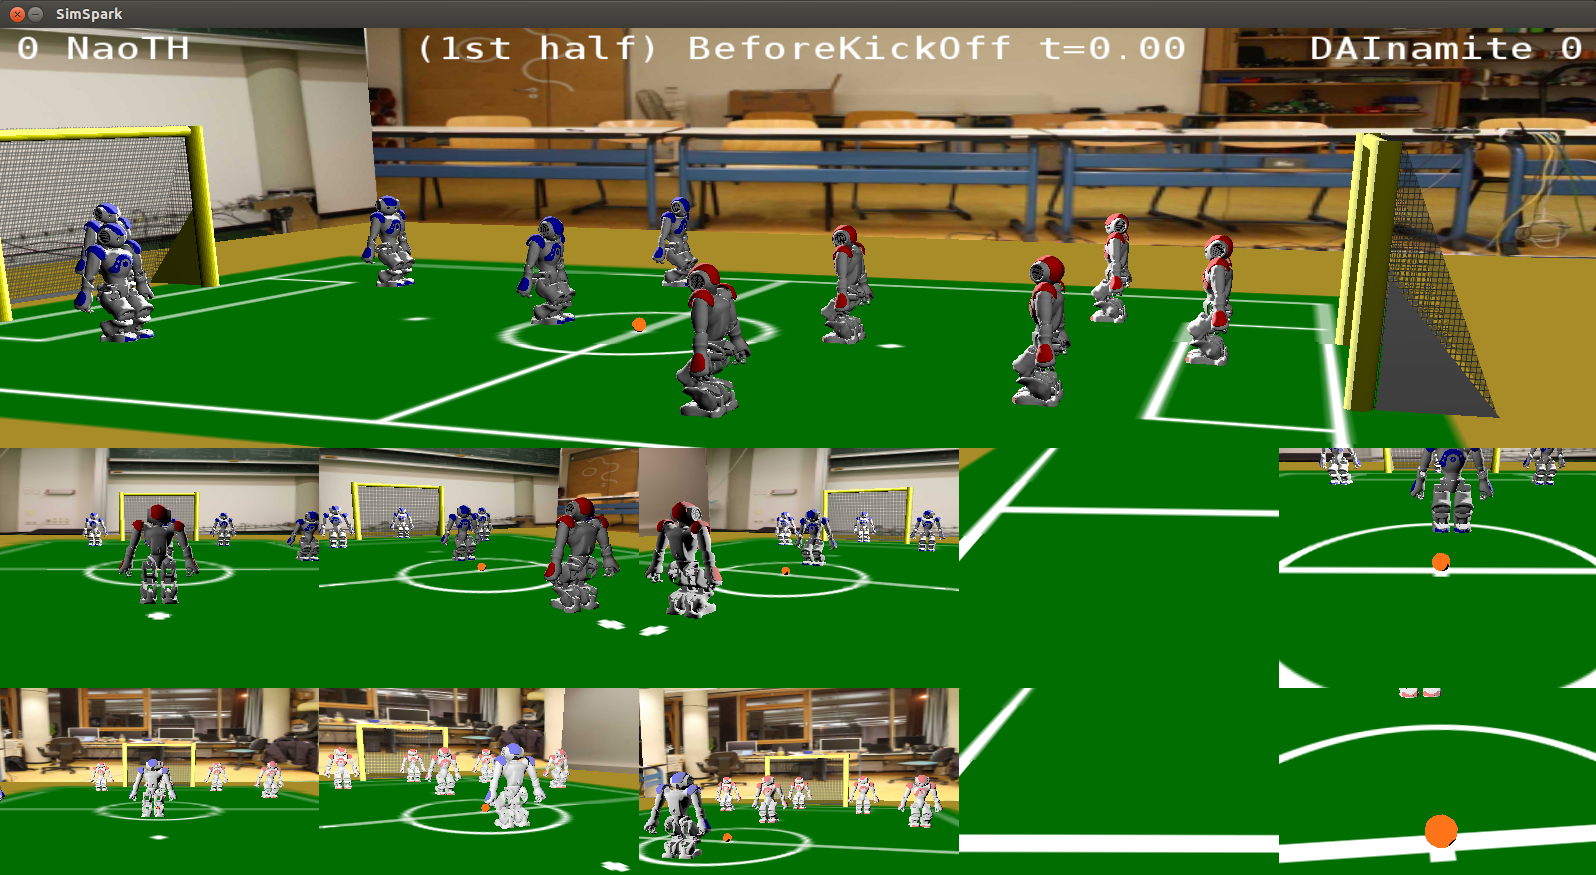
\includegraphics[width = 0.75\columnwidth]{simspark-spl}
  \caption{Prototype of the extended SimSpark for Standard Platform League.
    The bottom of screen are images of robot cameras.}
  \label{f:simspark-spl}
\end{figure}

\paragraph{RoboCup Soccer Humanoid League}
Of course the simulator can also be extended for other leagues by adding new robot models.
For example, in RoboCup Humanoid Kid Size League, FUmanoid\cite{Donat2012} uses
SimSpark to perform multi-level testing methods for archiving higher
quality in each module of their robot control software and unlink the
module test from the robotic hardware.


\section{Conclusion and Future Work}
\label{s:conclusion}
SimSpark is a powerful tool to state different multi-robot researches.
The introduction of a humanoid robot model to the simulation gave another perspective to the league.
The interest in the 3D simulation competition is growing fast and research is slowly getting back to the design and implementation of multi-agent higher-level behaviors based on solid low level behavior architectures for realistic humanoid robot teams.

SimSpark has undergone continuous development driven by the requirement of continues research in multi-robot system.

\paragraph{Integration With Existing Robotic Frameworks}
To enhance the usability of SimSpark for wider usage, and also to make it easier
for developers to develop and test their robotic software on SimSpark and to
use the same code on real hardware, we aim to integrate SimSpark to an 
existing robotic framework. Player is a well-known robotic framework which
can be used to control both real and simulated robots. We planned to integrate
SimSpark with Player so that people can develop agents for SimSpark using 
Player interfaces. It has the additional benefit of using Player's network
protocol which is much more efficient than the current network protocol used
in SimSpark. It is also a good opportunity to enhance the multi-threaded 
capabilities of SimSpark given the asynchronous nature of using Player with
different robot sensors. 

Recently, another robotic framework called ROS is gaining popularity and is in
active development. Therefore, we will reconsider our planning and might decide
to integrate SimSpark with ROS instead. However, considering that Player itself
is integrated into ROS, integrating with Player still might make sense. 

If SimSpark is integrated into an existing robotic framework, it is possible 
for researchers to develop a single program to control both a simulated 
robot inside and the same real robot given that the robot itself is also
supported by the framework. It will be also much easier to attract people 
who have developed programs for real robots using the framework to experiment
with SimSpark.

\paragraph{physics simulation engine abstraction / Bullet}
\paragraph{more robot models, formate?}
\section*{Acknowledgments}
We wish to thank other members in in the Maintenance Committee of the RoboCup Soccer Simulation League, especially the original authors of SimSpark: M. K\"ogler, M. Rollmann, and O. Obst. Furthermore, thanks go to J. Boedecker for introducing us to the SimSpark project.\todo{other names here...}
\bibliographystyle{splncs03}
\bibliography{reference}
\end{document}
